\chapter{IRT item parameter calibration in Julia} % Main chapter title
\label{sec:Julia}

Item response theory (IRT) models, already introduced in Chapter \ref{sec:TestTheories}, are a class of statistical models which are intended to describe the response behaviors of individuals to a set of questions which have a discrete outcome. The item responses are observable manifestation of underlying traits or constructs not directly measured which are called \emph{latent} variables. In the framework of latent class analysis IRT models hyphotesize the latent variable as continuous, instead, the observed variables are patterns of discrete-valued responses, in particular they can be dichotomous (correct/incorrect) or polythomous. Common assumptions in IRT are the unidimensionality of the latent trait is  since it's considered to be enough to describe the individuals propensity to endorse the items in the survey and conditional indipendence of the probability of a correct response given a certain level of ability. Moreover, IRT models can be seen as a specific type of fixed-effect or random-effect model \parencite{fox2006fixed} or, changing the parametrization, they become a particular case of latent regression models \parencite{von2010stochastic}. 

Once the model is set, the parameters and the latent variables must be estimated. For example in the 2-parameter logistic (2PL) model \parencite{BockMislevy1982}, easiness and discrimination power of the items must be quantified. Several algorithms to retrieve the estimates exist, most of them are based on the expectation maximization (EM) paradigm and differ on the way in which the expectation is approximated and in how the optimization model is solved, some examples are the joint maximum likelihood (JML)\parencite{lord1968statistical}, the marginal maximum likelihood (MML) \parencite{drasgow1989evaluation}, the stochastic EM algorithm \parencite{fox2003stochastic} and the Bayesian methods which adopt monte carlo Markov chain (MCMC) or Gibbs samplers technique to approximate and maximize the posterior of the latent variable \parencite{matteucci2012prior}. 

In this work the unidimensional model, dichotoumous response data and MML estimation method will be taken into account. The latter is widely recognized to outperform the JML and MCMC in terms of consistency of the estimates \parencite{andersen1977sufficient, neyman1948consistent} and computational time  \parencite{patz1999applications} respectively. Unlike the joint maximum likelihood estimation technique, which treat each of the responses as separate observational units, the MML estimation treats only the individuals as such. To accomplish this the MML technique assumes that the latent traits are random effects sampled from some continuous distribution, usually discretized in order to compute the expected value of the likelihood in the first step of the EM algorithm, called \emph{E-step}. In this context, the latent regression representation allows to perform faster computations of the involved functions since some arrays are computed only once and reused in all the iterations. Another advantage is the use of simple linear algebra transformation such as matrix/matrix or matrix/vector multiplications which are extremely fast in modern programming languages\footnote{The \texttt{BLAS} routines are an example of very fast implementation of linear algebra operations. See  \url{http://www.netlib.org/blas/}}. 

Moreover, since we chose to work in the \texttt{Julia} environment due to its suitability for numerical and computational tasks, we also developed a calibration algorithm for the case of the unidimensional 2PL already introduced in \ref{ch:ATA}. The cubic-spline interpolation-extrapolation method \parencite{birkhoff1960smooth} is used to recompute the masses of the rescaled observed ability distribution at the predefined theta points. The details of the applied methodology are provided in Section \ref{sec:estimation} together with a software benchmarking which compare the performance of our algorithm to the \texttt{R} \texttt{mirt} package.

Finally, a full reading of this chapter will suggest to both practitioners and scholars a framework for building a pre-test design without knowing the item parameters and for doing a simulation study for testing the performance of an estimation method. The framework is described in Section \ref{sec:Julia:simSet}. All the code is available at \url{https://github.com/giadasp/Calibration}.


\section{MML Estimation}\label{sec:estimation}

Test assembly models might be based on CTT or IRT item parameter estimates. In order to compute these values, a test assembler needs to perform what is called, a \emph{calibration} of the items. Here, the objective is achieved using the Expectation-Maximization (EM) paradigm in which the M-step is done by maximizing the likelihood marginalized with respect to the distribution of the initialized abilities. The model is described in \textcite{bock1981marginal}. We do not use the approach based on response patterns because we allow an unbalanced design of the pre-test after which the calibration takes place.

The algorithm requires just to input the responses of the test-takers, and since we allow for an unbalanced design, the data frame can contain missings. All the others input have a default value which can be  modified, in particular, the user can define\footnote{Default values can be found in the file \texttt{structs.jl} in the Github page}: the number quadrature points, $K$, in which approximate the integral of the ability distribution, the bounds for the ability distribution or starting knots and masses, starting points and bounds for the item parameters. The user can also define the features of the external EM algorithm and of the internal M-step, here called respectively \texttt{external and internal optimizations}, such as the stopping criteria. 

In details, our EM algorithm is composed of an iterative scheme. At the beginning of each iteration, the classical E-step and M-step are resolved; there follows a phase of readjusting and rescaling of the masses of the latent distribution. When at least one stopping criterion is met, the abilities of the test-takers are estimated. Before comprehensively outlining the mentioned stages we introduce the notation used in the next paragraphs.
Given a set of $N$ respondents and $I$ items in a pool, we want to estimate a set of vectors $\boldsymbol{\xi}_i$ of length $nPar$ of item parameters from a matrix $\mathbf{U}=\{u\}_{i,n}$ of dichotomous responses, i.e.

$$u_{i,n}= 
\begin{cases} 
1, & \mbox{if the test taker $n$ answered correctly to the question $i$}  \\
0, & \mbox{if the test taker $n$ answered incorrectly to the question $i$}\\
missing, & \mbox{if the item $i$ hasn't been administered to the test taker $n$,}
\end{cases}
$$

where $i=1,\ldots,I$ and $n=1,\ldots,N$. For example if the chosen model is the 2PL we will have $nPar=2$, instead for the 1PL model $nPar=1$.
For simplicity we will also define the vectors $\mathbf{u}_i$ and $\mathbf{u}_n$ rispectively as the $N$ rows and the $I$ columns of the matrix $\mathbf{U}$. 
The density of the latent variable $\theta$, the prior in a Bayesian perspective, is denoted by $p(\theta|\boldsymbol{\tau})$ where the vector $\boldsymbol{\tau}$ contains the parameters which characterize its probability distribution. In order to compute the expectation of the complete log-likelihood which consists of a complex integral, a discretization of the distribution is performed at $K$ knots in the domain of $\theta$, namely the $X_k$s for $k=1,\ldots,K$. Since, most of the times, the latent density is not known, for each of these points the mass $W_k$ is initialized to the value of an arbitrarily reasonable probability density (the observed empirical distribution of a previous test administration may be used) and readjusted in the calibration process to match the distribution of the ability in the population under examination.

\subsection{E-step} 

In practice, in the E-step the expected value $E_{\theta|u}\left[\mathit{l}(\boldsymbol{u},\theta|\boldsymbol{\xi})\right]$ of the complete data log-likelihood is computed by summing the log-likelihoods of the $I$ items weighted by the posterior distribution  $p(X_k|\boldsymbol{u}_n,\boldsymbol{\tau},\boldsymbol{\xi})$ of the latent variable: 
\begin{equation}\label{eq:expect}
\begin{aligned}
 E_{\theta|u}\left[\mathit{l}(\boldsymbol{u},\theta|\boldsymbol{\xi})\right] & =\sum_{i=1}^{I}{ \sum_{n \in n_i}{\int_{\theta}{\left[\mathit{l}(u_{i,n}|\theta,\boldsymbol{\xi}_i)+\log(p(\theta|\boldsymbol{\tau}))\right]p(\theta|\boldsymbol{u},\boldsymbol{\tau},\boldsymbol{\xi})} d\theta}} \\
 & \approx \sum_{i=1}^{I}{\sum_{n \in n_i}{\sum_{k=1}^K {p(X_k|\boldsymbol{u}_n,\boldsymbol{\tau},\boldsymbol{\xi})\left[\mathit{l}(u_{i,n}|X_k,\boldsymbol{\xi}_i)+\log(p(X_k|\boldsymbol{\tau})) \right]}}} \\
 & \approx \sum_{i=1}^{I}\sum_{n \in n_i}{\sum_{k=1}^K {{\color{DarkCyan}p(X_k|\boldsymbol{u}_n,\boldsymbol{\tau},\boldsymbol{\xi})\mathit{l}(u_{i,n}|X_k,\boldsymbol{\xi}_i)}}} \\
 & +{\color{Indigo}p(X_k|\boldsymbol{u}_n,\boldsymbol{\tau},\boldsymbol{\xi})\log(p(X_k|\boldsymbol{\tau}))} \\
 & =\sum_{i=1}^{I}{\sum_{n \in n_i}{\sum_{k=1}^K{{\color{DarkCyan}Q(u_{i,n}|X_k)}+{\color{Indigo}\phi(X_k|\boldsymbol{\tau})}}}},
\end{aligned}
\end{equation}
where
\begin{equation}\label{eq:expectation}
\begin{aligned}[c]
p(X_k|\boldsymbol{u}_n,\boldsymbol{\tau},\boldsymbol{\xi}) & = \frac{W_k\left[ \prod_{i \in i_n}{L(u_{i,n}|X_k,\boldsymbol{\xi}_i)}\right]}{\sum_j{W_j \ \left[ \prod_{i \in i_n}{L(u_{i,n}|X_j,\boldsymbol{\xi}_i)}\right]}} \\
& = \frac{W_k \ \exp\left[ \sum_{i \in i_n}{\mathit{l}(u_{i,n}|X_k,\boldsymbol{\xi}_i)}\right]}{\sum_j{W_j \ \exp\left[ \sum_{i \in i_n}{\mathit{l}(u_{i,n}|X_j,\boldsymbol{\xi}_i)}\right]}}, \\
\mathit{l}(u_{i,n}|X_k,\boldsymbol{\xi}_i) &=u_{i,n} \Psi(\boldsymbol{\xi}_i| X_k)-\log(1+\exp(\Psi(\boldsymbol{\xi}_i|X_k)))
\end{aligned}
\end{equation}
and $\Psi(\boldsymbol{\xi}_i| X_k)$ is the linear function proper of the latent regression models. For example, in case of the 2PL model, $\Psi(\boldsymbol{\xi}_i|X)=b_i+a_iX$.

To simplify the notation we will write $\mathit{L}_n(X_k,\boldsymbol{\xi})$ in place of $ \exp\left[ \sum_{i \in i_n}{\mathit{l}(u_{i,n}|X_k,\boldsymbol{\xi}_i)}\right]$ and $\mathit{l}_n(X_k,\boldsymbol{\xi}_i)$ for its logarithmic transformation.



\subsection{M-step}
Noticing that the function \eqref{eq:expectation} is separable with respect to the $I$ items, the M-step is performed individually for each item $i$. In the $s$-th iteration the estimates of the item parameters of item $i$ are obtained by maximizing the just defined expected log-likelihood:

\begin{equation}\label{eq:M-step}
\begin{aligned}[c]
& \hat{\boldsymbol{\xi}}_i^{(s)} && \quad = \text{arg}\max_{\boldsymbol{\xi}_i} \quad &&  E_{\theta|u}\left[\mathit{l}(\boldsymbol{u},\theta|\boldsymbol{\xi})\right]_i \\
& && && \approx \sum_{k=1}^K{\sum_{n \in n_i}{Q(u_{i,n}|X_k)}} \\ 
& && && \approx \sum_{k=1}^K\sum_{n \in n_i}{p(X_k|\boldsymbol{u}_n,\boldsymbol{\tau},\hat{\boldsymbol{\xi}}^{(s-1)})\mathit{l}(u_{i,n}|X_k,\boldsymbol{\xi}_i)} 
\end{aligned}
\end{equation}

The maximization is usually performed numerically by using non-linear solvers. In \texttt{Julia} several high-level interfaces are available to communicate with a multitude of solvers, from commercial, such as Artelis Knitro or Fico Express, to open-source, like NLopt and Ipopt \footnote{\url{http://www.juliaopt.org/JuMP.jl/v0.20.0/installation/}}.

\subsection{The rescale of the latent distribution}

The posterior distribution depends on the item parameters estimated at the prevoous step $s-1$ and to the masses $W_k$. The latters can be constant of may be adapted at each iteration of the EM algorithm. Since the model is identified only if the metric of the latent probability distribution is fixed (for example having mean zero and standard deviation one), the adaptation of the masses is a very delicate phase very subject to unstable results. Usually, the starting points for the masses come from the probability density function of the standardized Normal, but they can be arbitrarily initialized. After the first iterations, the $W_k$ may be adapted by using the approach introduced by \textcite{mislevy1984estimating}:

\begin{equation}\label{eq:maxWk}
\sum_{n \in n_i}{\log{\sum_{k=1}^K{{\mathit{L_n}(X_k,\boldsymbol{\xi})}W_k}}} 
\end{equation} 

and adding a Lagrange multiplier to constrain the sum of the masses to be equal to $1$. 
Practically, the optimal weights are analytically computed as the average of the posterior distribution among the $N$ respondents: 

\begin{equation} \label{eq:updateWk}
W_k^{(s)}  = 1/N \sum_{n=1}^N{p(X_k|\boldsymbol{u}_n,\boldsymbol{\tau},\hat{\boldsymbol{\xi}}^{(s)})} 
\end{equation}

After the masses have been adjusted, it is necessary to rescale the quadrature points in order to match a predefined metric which consists of: mean, $\mu_\theta$, and standard deviation, $\sigma_\theta$. At the iteration $s$, the rescale is performed by generating new knots $\boldsymbol{X}^{*(s)}=\{X_1^{*(s)},\ldots,X_K^{*(s)}\}$ by linearly transform the original quadrature points $\boldsymbol{X}^{(s)}=\{X_1^{(s)},\ldots,X_K^{(s)}\}$ as follows,

\begin{equation}\label{eq:rescale}
X_k^{*(s)}=\frac{(X_k^{(s)}-(\boldsymbol{W}^{(s)'}\boldsymbol{X}^{(s)}-\mu_\theta))\sigma_\theta}{\sqrt{\boldsymbol{W}^{(s)'}(\boldsymbol{X}^{(s)}\odot \boldsymbol{X}^{(s)})}}, \quad  k=1,\ldots,K;
\end{equation}

where $\boldsymbol{X} \odot \boldsymbol{X}$ is simply a vector containing the squares of the elements of $\boldsymbol{X}$. $\boldsymbol{W}^{(s)}$ comes from the EM algorithm as the optimum of \eqref{eq:maxWk}.
Using the new quadrature points in the next iterations is not advisable because they can alter the convergence of the algorithm and they can gradually translate outside a reasonable interval of variation of the ability. To overcome this issue the \texttt{R} package \texttt{mirt} adopts the interpolation/extrapolation approach introduced by \textcite{woods2007} that linearly estimates new weights $\boldsymbol{W^{*(s)}}$ on the original quadrature points $\boldsymbol{X}^{(s)}$. 

In this work, the spline interpolation is considered (see \textcite{de1978practical} for a gentle introduction and \textcite{meijering2002chronology} for a historical traceback) add applied to calibration problems by using the \texttt{Julia} package \texttt{Interpolations.jl}\footnote{\url{https://github.com/JuliaMath/Interpolations.jl}}.
In particular, by this package, it is possible to choose between linear, quadratic, and cubic interpolation; on-grid and on cell interpolation objects and flat, line, free, periodic and reflect boundary conditions. After several trials, the \textbf{cubic-spline,} with on-grid interpolation and line boundary condition is selected because it had the combination which produced lower RMSEs of the estimates.

This step is performed only in the first iterations in order to avoid an undesired behaviour of the spline and a lack of convergence of the EM procedure, in particular the masses are adapted and rescaled in iterations $3,6$ and $9$.

\subsection{Ability estimation}


Once the $\hat{\boldsymbol{\xi}}_i^{(s)}$ have been obtained and the weights $\boldsymbol{W}^{(s)}$ have been updated, if no prior has been chosen, the $\hat{\theta}_n^{(s)}$ can be estimated by using the expected a posteriori (EAP, \textcite{BockMislevy1982}) or maximum a posteriori (MAP) method as follows:
\[\hat{\theta}_n^{(s)}{}_{EAP}=\sum_k{p(X_k|\boldsymbol{u}_n,\boldsymbol{\tau},\hat{\boldsymbol{\xi}}^{(s)})X_k},\]

\[\hat{\theta}_n^{(s)}{}_{MAP}=\{X_k : k=\text{arg}\max_k p(X_k|\boldsymbol{u}_n,\boldsymbol{\tau},\hat{\boldsymbol{\xi}}^{(s)}) \}.\]

However, if a prior $p(\theta|\boldsymbol{\tau})$ is selected, the latter is transformed into:

\begin{alignat*}{3}
& \hat{\theta}_n^{(s)}{}_{MAP}&&=\text{arg}\max_\theta p(        \theta|\boldsymbol{u}_n,\boldsymbol{\tau},\hat{\boldsymbol{\xi}}^{(s)}) \\
& &&=\text{arg}\max_\theta \mathit{l}(u_{i,n}|\theta,\boldsymbol{\xi}_i)+\log(p(\theta|\boldsymbol{\tau})).
\end{alignat*}
\color{black}

\subsubsection{The algorithm}

We optimize the marginal likelihood by using the \texttt{NLopt.jl} package based on the \texttt{NLopt} suite, in particular, we use the \texttt{SLSQP} algorithm, which is fast and stable. The implemented EM sub-routine is described in the following pseudo-algorithm:

\begin{algorithm}[ht]
	\caption{EM}\label{alg:EMalg}
	\begin{algorithmic}
		\State Initialize $\boldsymbol{\xi},\boldsymbol\theta$ to arbitrary values (e.g. $b^{(o)}_i=0.0$, for all $i$)
		\State Initialize $\boldsymbol{W}$ by the Normal$(0,\sigma_\theta)$ density.
		\State s=1
		\While{none of the stopping criterion is satisfied}
		\State E-step: Compute \eqref{eq:expectation} $\rightarrow$ $p(X_k|\boldsymbol{u}_n,\boldsymbol{\tau},\boldsymbol{\xi}), \quad \forall n,k$
		\State M-Step: Maximise \eqref{eq:M-step} by \texttt{Nlopt} $\forall i$ $\rightarrow$ $ \hat{\boldsymbol{\xi}}^{(s)}$
		\If{(s==9 or s==12 or s==15)}
		\State Update $\boldsymbol{W}$: Compute \eqref{eq:updateWk} $\rightarrow$ $\boldsymbol{W}^{*(s)}$
		\State Rescale $\boldsymbol{X}$: Compute \eqref{eq:rescale} $\rightarrow$ $\boldsymbol{X}^{*(s)}$
		\EndIf
		\State Interpolate: Cubic-spline of $\boldsymbol{W}^{*(s)}$ on  $\boldsymbol{X}$ $\rightarrow$ $\boldsymbol{W}^{(s)}$
		\State s+=1 
		\EndWhile
	\end{algorithmic}
\end{algorithm}

\subsection{Bootstrap}\label{sec:juliaBS}

The strength of IRT models, theoretically, is to have invariant item parameters across samples of examinees from the same population. Practically, invariance is hard to be guaranteed under the calibration process. 
Several factors may contribute to obtaining considerably different item parameter estimates from the same set of items under different conditions. Such factors include the positioning of items in the test, different populations, different points of time. In \textcite{tsutakawa1990effect} is showed that using estimates of item parameters instead of their actual values could lead to biases in the following inference about the students' ability. Also, \textcite{veldkamp2013application} pointed out that an item selection based on maximum information would capitalize on positive estimation errors if the uncertainty in the estimates of discrimination parameters is not taken into account. 

Although existing methods for handling uncertainty in item parameters provide a variety of tools, most of them belong to Bayesian applications, which need to know the prior distribution of item parameters and abilities. An alternative approach that simulates the calibration under different conditions and that does not ask to assume any probability distribution is the \emph{bootstrap} \parencite[see]{efron1993}. In particular, we performed the calibration in a large number of resamples of the response data. The aim is to fully characterize the uncertainty related to each item parameter estimates by exploring its empirical distribution function (edf). 

Given an item bank of items and a sample of students, from here called \emph{full sample}, after the items have been administered, we have a matrix of dichotomous responses. For each item, we want to estimate a vector $\hat{\xi}_i$ of IRT parameters which may contain a different number of parameters in case we have a different model such as the 1PL, the 2PL or the 3PL. 
We first perform an \emph{overall calibration} (on the full sample of students) by following the marginal maximum likelihood estimation method (MMLE) \textcite{bock1981marginal}, already presented previously. Once the overall estimates of item parameters and abilities of the students are obtained, we proceed with resampling eith replacement $N^* = N$ rows of the response matrix, $R$ times, and, in each of these replications we reestimate the IRT item parameters. In this way we have $R$ samples of each item parameter. 

Depending on the way the responses are resampled we can distinguish two different algorithm: the parametric and the non-parametric schemes. They are described analitically in the next paragraphs.

\subsubsection{Non-parametric bootstrap}

\begin{algorithm}[h]
	\caption{Non-parametric bootstrapped calibration}
	\begin{algorithmic}
		\State Choose a large number of repetitions $R$, the subsample size $N^* = N$ and an ability point $\theta_0$ in which maximize the TIFs.
		\For{$r=1:R$}
		\State Sample with replacement $N^*$ rows of the responses matrix assuming that each row has a $1/N$ probability to be drawn. 
		\State Calibrate the items in the subsample. Get $\hat{\xi}_{r}=\{\hat{\xi}_{1r},\ldots,\hat{\xi}_{Ir}\}$.
		\State Compute the IIF for each item for a chosen set of ability points $\mathbb{\theta}_0$ using $\hat{\xi}_{ir}$.
		\State Store the vectors $\hat{\text{IIF}}(\theta_0)_{r}=\left\{\hat{\text{IIF}}(\theta_0)_{1r},\ldots,\hat{\text{IIF}}(\theta_0)_{Ir} \right\}$
		\EndFor
	\end{algorithmic}
\end{algorithm}

\subsubsection{Parametric bootstrap}\label{sec:parbs}
\begin{algorithm}[h]
	\caption{Parametric bootstrapped calibration}
	\begin{algorithmic}
		\State Choose a large number of repetitions $R$, the subsample size $N^* = N$ and an ability point $\theta_0$ in which maximize the TIFs.
		\State Estimate $\boldsymbol{\hat{\xi}}$, $\hat{\boldsymbol{\theta}}$ and $\mathbf{\hat{W}}$ on the full sample.
		\State Discretize the distribution of the ability by dividing its continuum in $K$ bins and approximate the probability of sampling the $n$-th examinee by its relative frequency $\hat{p}_n$ of his $\hat{\theta}_n$ assuming that, in each bin, the students (and their abilities) are uniformely distributed.
	\For{$r=1:R$}
	\State Resample with replacement from the discretized distribution, $N^*$ rows from the responses matrix.  
		\State Calibrate the items in the subsample taking $\mathbf{\hat{W}}$ as fixed and equal to its overall estimate. Get $\hat{\xi}_{r}=\{\hat{\xi}_{1r},\ldots,\hat{\xi}_{Ir}\}$.
		\State Compute the IIF for each item for a chosen set of ability points $\mathbb{\theta}_0$ using $\hat{\xi}_{ir}$.
		\State Store the vectors $\hat{\text{IIF}}(\theta_0)_{r}=\left\{\hat{\text{IIF}}(\theta_0)_{1r},\ldots,\hat{\text{IIF}}(\theta_0)_{Ir} \right\}$
		\EndFor
	\end{algorithmic}
\end{algorithm}

\section{Simulation study}

In order to show the suitability of \texttt{Julia} as a programming language for calibration purposes we present a benchmark analysis between our application and other open-source frameworks, such as the \texttt{R} programming language.
In particular, we focused on the \texttt{mirt}\texttt{R} package \parencite{R,JSSv048i06} because we believe it is the most reliable and fast open-source software for this task. 
Other open-source options available for items calibration were: the \texttt{R} package \texttt{ltm} \parencite{JSSv017i05} and \texttt{stan} \parencite{JSSv076i01} from a Bayesian perspective. The first, as far as we know, doesn't handle the missings coming from an unbalanced pre-test design, the second produced unstable results. Both were very slow compared to \texttt{mirt}.

All the tasks are performed using \texttt{Julia 1.2.0} and \texttt{R 3.6.1} and working on a desktop computer with the following features: Windows 10, Intel-core i5-4670 CPU and 16GB of ram.

Specifically, the comparison is made between \texttt{Julia} and two versions of the algorithm implemented in \texttt{mirt}. About \texttt{mirt}, the first version uses the default of the argument \texttt{dentype}, which rules the type of density that is used for the latent trait parameters, i.e., the Gaussian density. The second version, named here \texttt{mirt EHW},  estimates the latent distribution with the empirical histogram and interpolation extrapolation method described in \textcite{woods2007}. The unidimensional 2PL model has been chosen for the simulation together with dichotomous observed response variables.
Through the analysis of the simulation results, first, the accuracy of estimates, in terms of BIAS and RMSE, and computational performance are evaluated for the three softwares in all the cases defined in \ref{tab:casesJulia}. Secondly, a non-parametric and parametric bootstrap is applied on the calibration process for the standard setup in order to characterize the uncertainty related to the estimates and to illustrate their sampling distributions.

\subsection{Simulation settings (Framework for pre-testing)} \label{sec:Julia:simSet}
\label{sec:sim_catbs}
Several simulations are performed. Each design is driven by a different combination of variables that may recreate real pre-test situations. The aim of this section is not only to describe the process in which we benchmarked the mentioned algorithms but also to give to potential users an efficient framework for developing a test assembly strategy, from the assembly of the pre-tests to the calibration of item parameters. 
In practice, we chose to fix the length of the test at 50 items, $I=250$, and we varied the other variables as follows:
	\renewcommand{\arraystretch}{1.3}%
\begin{table}[ht]
\centering
\caption{Simulated  distributions for item parameters and \hspace{10pt}  ability \label{tab:combJulia}}
	\begin{tabular}{ l  c }
		\toprule
		$b$         & $  \text{Normal}(0,1), \ \text{Uniform}(-4,4)  $ \\%[5pt]
		$a$         & $  \text{LogNormal}(0,0.5), \ \text{Uniform}(0.001,4) $ \\%[5pt]
		$\theta$    & $\text{Normal}(0,1), \ \text{LogNormal}(0,0.25)$ \\%[5pt]
		$N$                             & 600, 3000, 6000 \\%[5pt]
		\bottomrule  
	\end{tabular}
\end{table}

The distributions of the item parameters and the ability have been chosen according to the literature \parencite[see for example]{glas2005modeling, glas2005testing, ban2002data}.
We decided to include a case plausible in the real world, that is the case 2b where the abilities of the test-takers will be drawn from a LogNormal(0,0.5) and then changed of sign in order to increase the probability of having lower high-performing examinees. 

	\renewcommand{\arraystretch}{1.3}%
Next table details all the examined cases:
\begin{table}[htpb]
\centering
\caption{Simulation settings \label{tab:casesJulia}}

	\begin{tabular}{ l c c c c  }
		\toprule
		\#case     & $b$ & $a$ & $\theta$ & $N$ \\%[5pt]
		\midrule
		1a    & $N(0,1)$ & $\text{LogN}(0,0.25)$& $N(0,1)$ & $3000$ \\%[5pt]
		1b   & $N(0,1)$ & $\text{LogN}(0,0.25)$ & $N(0,1)$  & $600$ \\%[5pt]
		1c    & $N(0,1)$ & $\text{LogN}(0,0.25)$ & $N(0,1)$ &  $6000$ \\%[5pt]
		2a    & $N(0,1)$ & $\text{LogN}(0,0.25)$ & $\text{LogN}(0,0.5)$& $3000$\\%[5pt]
		2b    & $N(0,1)$ & $\text{LogN}(0,0.25)$ & $-\text{LogN}(0,0.5)$\footnote{The sampled abilities are changed in sign after being rescaled to the standard metric.}& $3000$\\%[5pt]
		3    & $N(0,1)$ & $\text{U}(0.001,4)$ & $N(0,1)$  & $3000$\\%[5pt]
		4    & $\text{U}(-4,4)$ &  $\text{LogN}(0,0.5)$& $N(0,1)$  & $3000$\\%[5pt]
		\bottomrule    
		
	\end{tabular}
	
\end{table}

The case n. 1a will be deeply explored since it is a standard-setting for calibration. We will call it the \emph{standard setup}.

Each step of the framework for the simulation study for the MML estimation is comprehensively described herewith:
\begin{enumerate}
	\item A combination of variables from Table \ref{tab:combJulia} and a metric are chosen. We decide to fix $\mu_\theta$ to $0$ and $\sigma_\theta$ to $1$.
	\item True values for $\boldsymbol\theta$ and $\boldsymbol{\xi}$ are sampled from the respective distributions. The simulated pool $\boldsymbol{\xi}^\dagger$ and abilities $\boldsymbol\theta^\dagger$ are linearly rescaled to fit the predefined metric. These quantities represent the true values in the benchmarking phase.
	\item To assemble the pre-test form, assuming no information is available about the IRT item parameters, we assign to each item an approximated easiness level, from 1 to 3. This information can be given by the experts of the domain of the item under examination. In this simulation the levels are approximated by cutting the sampled $b_i$s by the 25th, 50th and 75th percentiles of the true distribution of the easiness.
	\item $T=6$ tests are assembled with the following features: 10 anchor items, length = $50$, fixed difficulty (easiness) composition (25\%, 50\%, and 25\%) approximated by the three levels previously assigned. 
	The resulting pre-test design will be unbalanced. This means that the test forms are partially overlapped (presence of anchor items) and hence the response data will contain missings. To help understanding the structure of the design we define two types of design matrices: an \emph{items $\times$ tests} design matrix and a \emph{tests $\times$ examinees} design matrix. The first assigns the items from the pool to the tests; this is the result of the pre-test assembly. The second assigns the test forms to the test-takers. The combination of these two designs generates the \emph{items $\times$ examinees} design matrix. All these further configurations can be represented by a 0-1 matrix, respectively of sizes $I \times T$, $T\times N$ and $I \times N$. See figures \ref{fig:itemsxtests}, \ref{fig:testsxexaminees} and \ref{fig:itemsxexaminees} for a visual explanation. 	
	\item For each of the $S=100$ simulations, we use the \emph{items $\times$ examinees} design to generate the responses. One vector, $i_n$, for each test-taker and one vector, $n_i$, for each item are produced. They represent, in the same order, the indices where the columns and the rows of the \emph{items $\times$ examinees} design matrix are equal to $1$.
	For example, if the examinee $n$ takes the items $1$, $3$, $40$ and $52$, their vector $i_n$ will be equal to $\{1,3,40,52\}$. On the other side, if the item $i$ is given to the examinees $100$, $2540$ and $351$ its vector $n_i$ will be equal to $\{100,2540, 351\}$. These vectors are intensively used in the algorithm to filter the response matrix $\mathbf{U}$.
	The data matrices $\mathbf{U}_s$ will be generated by sampling, for each student $n$, a correct response to the item $i$ using a Bernoulli with a probability equal to
	
	\[P_{i,n}=\frac{1}{1+\exp{-(\Psi(\boldsymbol{\xi}_i^\dagger|\theta_n^\dagger))}} \]
	
	\item The calibration process is run for each of the $S$ simulations $\mathbf{U}_s$, for $s=1,\ldots,S$ by the EM algorithm \ref{alg:EMalg} and by the \texttt{mirt} package using the following settings:
	\begin{itemize}
		\item Bounds for $a$ and $b$ are $\{0,5\}$ and $\{-6,6\}$\footnote{\texttt{mirt} default solver which allows box bounds is \texttt{minlp}}. 
		\item Bounds for $\theta$ are $\{-6,6\}$. The quadrature is done on $K=61$ knots.
		\item Tolerance for the item parameters is $1e^{-4}$. Tolerance for the likelihood is $1e^{-8}$.
		\item The maximum number of iteration is set to $500$ and the time limit to $1000$ seconds.
	\end{itemize}
	\item The elapsed computational time and the RMSEs and BIASs for the estimated item parameters $\hat{\boldsymbol{\xi}}_s$ and individual abilities $\hat{\theta}_n$ across the $S$ simulations of response data are compared.
	
	Let $x_j^\dagger$ be the true value of the variable $x_j$ where $x$ can be an item parameter or the ability and the index $j$ may indicate a particular item or the test-taker Moreover, let $\hat{x}_{js}$ the estimates of the same variable in the $s$-th simulation, we define the RMSE and BIAS of the object $i$ as:
	
	\begin{equation}
	RMSE_j=\sqrt{\frac{1}{S} \sum_{s=1}^S{\left( \hat{x}_{js}-x_j^\dagger \right)^2}}
	\end{equation}
	\begin{equation}
	BIAS_j=\frac{1}{S} \sum_{s=1}^S{\left( \hat{x}_{js}-x_j^\dagger \right)}
	\end{equation}
	
\end{enumerate}


\subsection{Results} 

In the next sections, we illustrate the results of the calibration for the six cases under analysis calibrated using the three mentioned softwares \texttt{Julia} \emph{(jl)}, \texttt{mirt} with default settings (\emph{mirt}) and \texttt{mirt} with the Woods' empirical histogram (\emph{mirtEHW}).

First, the estimation accuracy of the algorithms is visually compared by analyzing the boxplotsof the RMSEs and BIASs, Figures \ref{fig:bpRMSE1a} and, \ref{fig:bpRMSE1b}, for the estimates of item parameters and abilities. In order to understand if the algorithms have a different behaviour at specific intervals of the domains we examinate also the scatter plots of the RMSEs and BIASs with respect to the true values, accordingly in Figures \ref{fig:spRMSE1a} and \ref{fig:spBIAS1a}. For the sake of brevity, in this chapter, only the complete results for the \emph{standard setup}, i.e. case 1a, are presented. On the other hand, the overall precision of each algorithms in all the cases is summarized in Tables \ref{tab:RMSE} and \ref{tab:BIAS}, where the RMSEs and BIASs are averaged across the item pool, for the item parameters, and across test-takers, for the abilities. For the plots of the other cases (from 1b to 4) please refer to Appendix \ref{ch:TablesAndFigures}.
Together with the precision of estimates, we intend to evaluate the computational performance of our implementation by comparing the elapsed time and the number of iterations observed for calibrating the items for all the algorithms.
Secondly, the estimated $\mathbf{\hat{W}}^{(s)}$, where $s=1,\ldots,S$, are plotted against the true $\mathbf{W}$ obtained by drawing 1.000.000 samples from the true distribution and computing the relative frequencies in the $K$ chosen $\mathbf{X}$ points.
In the last section, some examples of sampling distribution of the item parameters obtained by bootstrapping the calibration is reported. 

\subsubsection{Summary of estimation accuracy}
In the following tables the RMSEs and BIASs averaged across the item pool for discrimination and easiness parameters and across the test-takers for the latent variable are presented for all the cases under analysis. The lowest RMSEs and the BIASs most proximal to zero, i.e., the best achieved, are formatted in bold font. 
In the case of Normality of the latent trait (cases 1a, 1b and 1c) we can notice that the precision of the algorithms is almost the same for all the estimates except the \texttt{mirt\tiny{EHW}} which does not behave well in case of few observation, that is the case 1b in which $N=600$.
On the other hand, when it comes to have a non-Normal latent trait (case 2a and 2b) our algorithm has the best performance notably for the discrimination parameter in which the RMSEs are $0.01$ lower than the mirt package. No remarkable differences are observed in cases 3 and 4 where the distributions of the item parameters are different from the usual setting.
A substantial discrepancy is observed analysing the BIASs where our approach has a better overall performance.

\begin{table}[h]
	\centering
	\caption{RMSEs averaged across the item pool ($\hat{a}$ and $\hat{b}$) and test-takers ($\hat{\theta}$) \label{tab:RMSE}}
	\resizebox{\textwidth}{!}{
	\begin{tabular}{l  c c c | c c c | c c c   }
\toprule
		 & \multicolumn{3}{c|}{$\hat{b}$} & \multicolumn{3}{c|}{$\hat{a}$} & \multicolumn{3}{c}{$\hat{\theta}$} \\
		 case &jl & mirt &  mirt\tiny{EHW} &jl & mirt &  mirt\tiny{EHW} &jl & mirt & mirt\tiny{EHW} \\ 	
\midrule
1a &\textbf{0.114} &\textbf{0.114}& \textbf{0.114}& \textbf{0.134}&0.135 &0.135 &\textbf{0.311} &\textbf{0.311} &\textbf{0.311}   \\ 
1b &0.264 &\textbf{0.263} &0.877 & 0.339&\textbf{0.336} & 0.341& 0.320 & \textbf{0.317} &0.799\\ 
1c &\textbf{0.779} &\textbf{0.779} & 0.780&\textbf{0.094} &\textbf{0.094} &\textbf{0.094} &\textbf{0.310}& \textbf{0.310} &\textbf{0.310}  \\ 
2a &\textbf{0.111} & 0.117&\textbf{0.111} &\textbf{0.152} &0.166 & 0.154 & \textbf{0.294}& 0.333 & 0.315  \\
2b &\textbf{0.114} & 0.119 & 6.076 & \textbf{0.149} & 0.159 & 0.232 & \textbf{0.302} & 0.331 & 5.278 \\ 
3 &\textbf{0.138} &\textbf{0.138} &\textbf{0.138} &\textbf{0.214} &0.221 &0.227 &0.221 &\textbf{0.220} &\textbf{0.220}   \\ 
4 &\textbf{0.188}& 0.189&0.190 & \textbf{0.186}&\textbf{0.186}& 0.187&\textbf{0.372}& \textbf{0.372} &\textbf{0.372 }  \\ 
\bottomrule
	\end{tabular}
}
\end{table}

\begin{table}[h]
	\centering
	\caption{BIASs averaged across the item pool ($\hat{a}$ and $\hat{b}$) and test-takers ($\hat{\theta}$) \label{tab:BIAS}}
				\resizebox{\textwidth}{!}{
		\begin{tabular}{l  r r r | r r r | r r r   }
			\toprule
			 & \multicolumn{3}{c}{$\hat{b}$} & \multicolumn{3}{c}{$\hat{a}$} & \multicolumn{3}{c}{$\hat{\theta}$} \\
			case &jl & mirt &  mirt{EHW} &jl & mirt &  mirt{EHW} &jl & mirt &  mirt{EHW} \\ 	
			\midrule
			1a & \textbf{0.002} & 0.004 & \textbf{0.002} & \textbf{0.009} & 0.011 & 0.010 &{$2.8\times 10^{-4}$}  &-0.002 & {$\mathbf{2.0\times 10^{-4}}$}   \\ 
			1b & \textbf{0.005}& 0.006& 0.120&0.060 &\textbf{0.059} &0.642 & \textbf{-0.002}& -0.004&-0.105\\ 
			1c &\textbf{0.001 }&0.002 &\textbf{0.001} &0.005 &\textbf{0.004} &0.005 &{$-1.6\times 10^{-4}$}& {$-1.1\times 10^{-3}$}&{$\mathbf{1.5\times 10^{-4}}$}\\ 
			2a &\textbf{0.004} &-0.042 & 0.005& \textbf{0.005}&-0.091 &0.118 &{$\mathbf{4.8\times 10^{-4}}$} & -0.002 & -0.028  \\
 			2b &\textbf{-0.003}&0.040&6.073&\textbf{-0.009}&-0.072&0.006&{$\mathbf{9\times 10^{-4}}$}&-0.002&-5.268 \\ 
			3 & \textbf{0.001} &0.010 &\textbf{0.001} &\textbf{-0.013} &0.033 &0.044 &{ $\mathbf{3.9\times 10^{-4}}$}& -0.003& {$9.2\times 10^{-4}$}  \\ 
			4 &\textbf{0.001} & 0.006& \textbf{0.001}& \textbf{0.013}&\textbf{0.013} &0.014 &{$\mathbf{-7.1\times 10^{-5}}$} &{$-1.3\times 10^{-3}$} &{$2.2\times 10^{-4}$} \\ 
			\bottomrule
		\end{tabular}}
\end{table}

\subsubsection{The \emph{standard setup}}

\begin{figure}[h]
	\centering
	%\textbf{RMSEs of estimates with respect to the true values of item parameters and ability }\par\medskip
	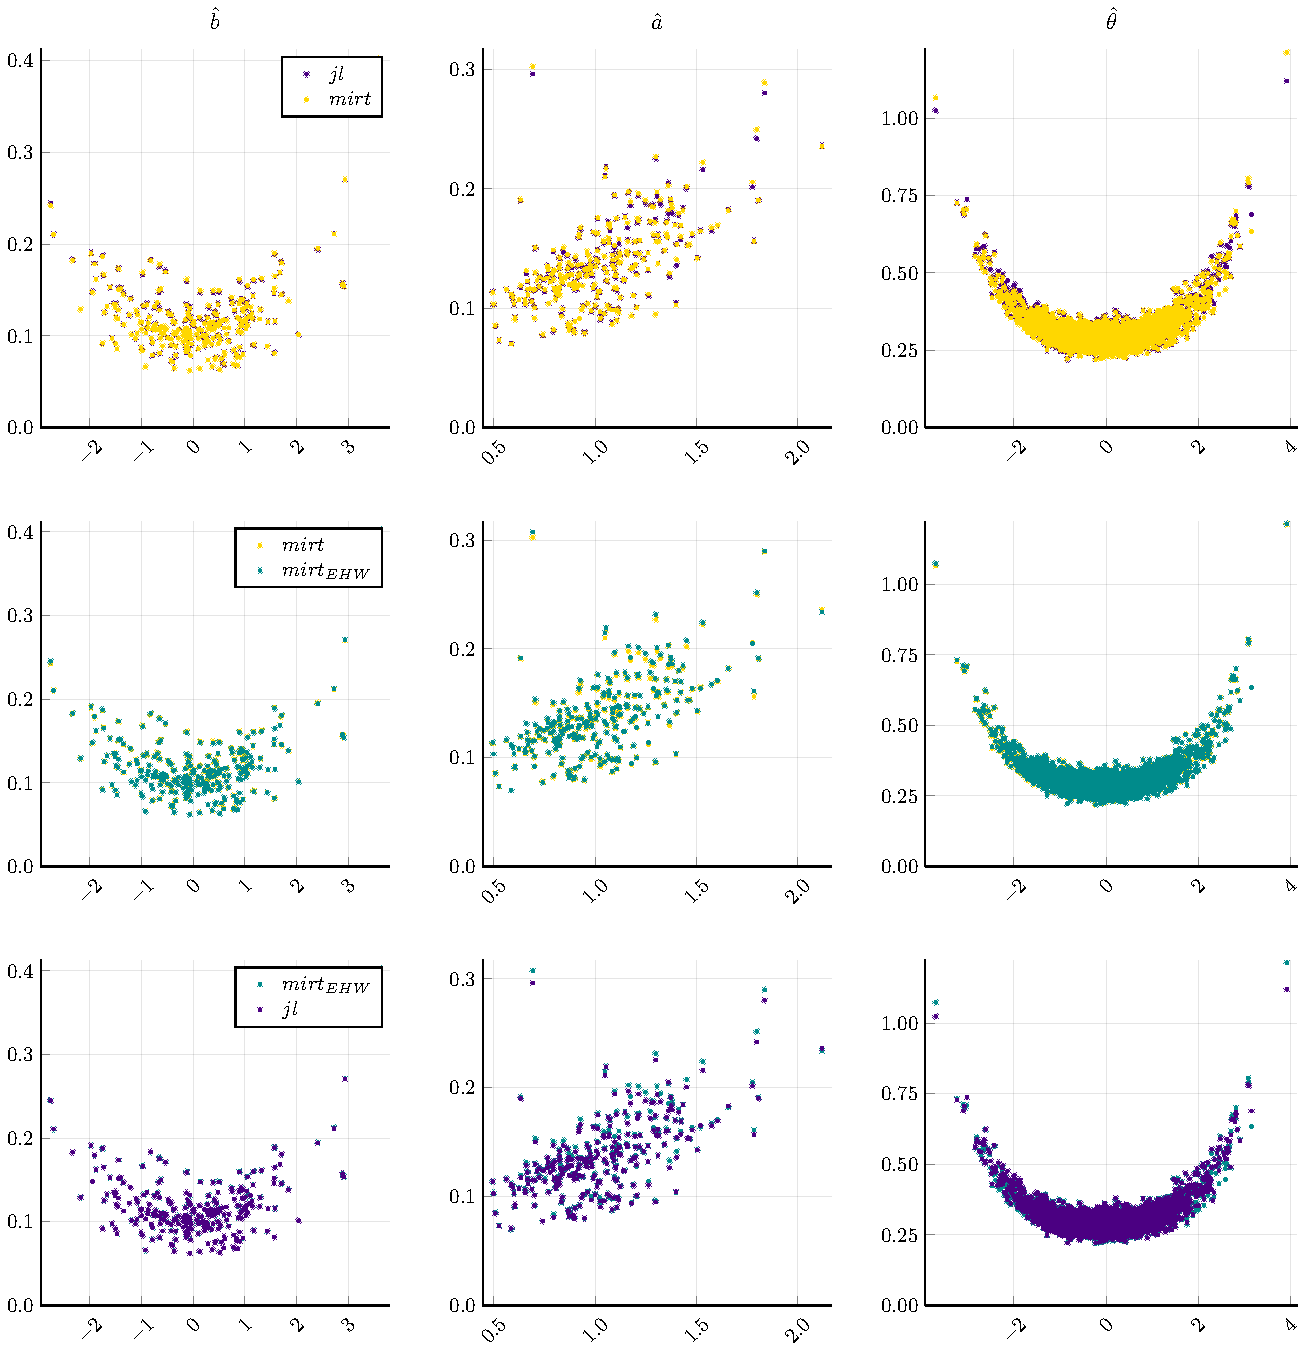
\includegraphics[width=\textwidth]{Figures/1/RMSEscatter.pdf}
	\caption{Case 1a - Scatter plots of RMSEs.}
	\label{fig:spRMSE1a}
\end{figure}
\begin{figure}[h]
	\centering
	%\textbf{BIASs of estimates with respect to the true values of item parameters and ability}\par\medskip
	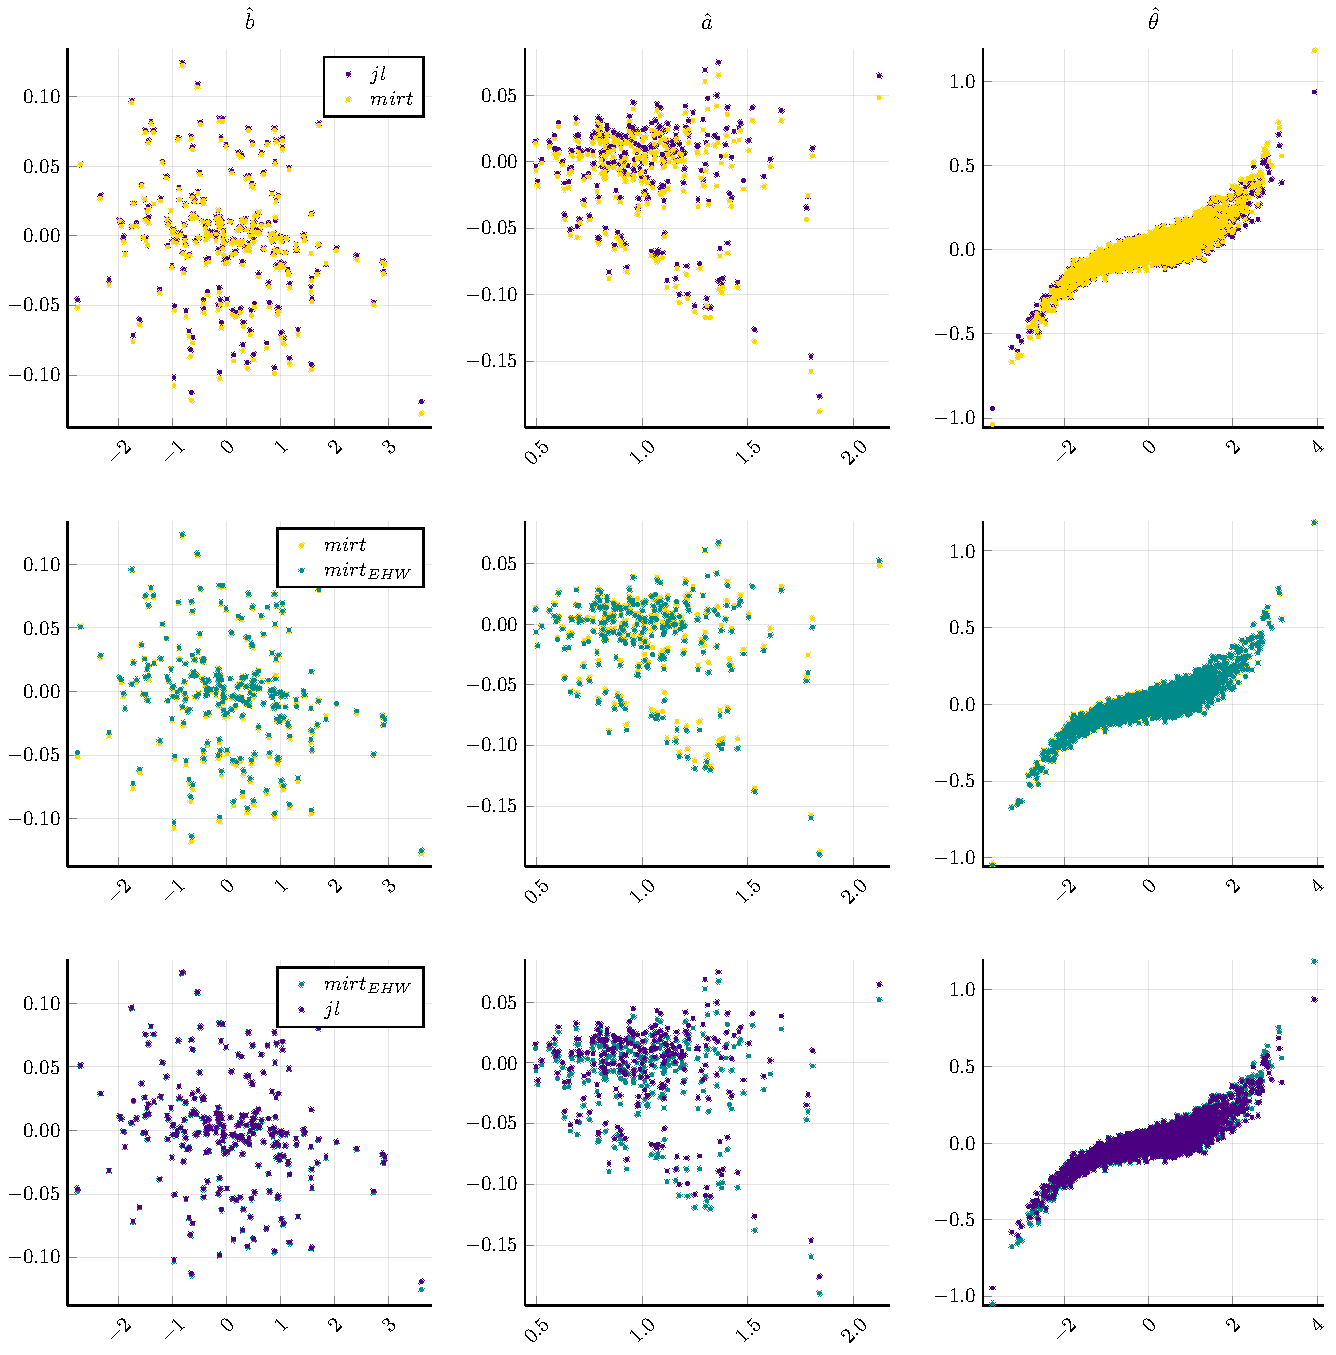
\includegraphics[width=\textwidth]{Figures/1/BIASscatter.pdf}
	\caption{Case 1a - Scatter plots of BIASs }
	\label{fig:spBIAS1a}
\end{figure}
\begin{figure}[h]
	\centering
	\begin{tabular}[b]{c c c}
		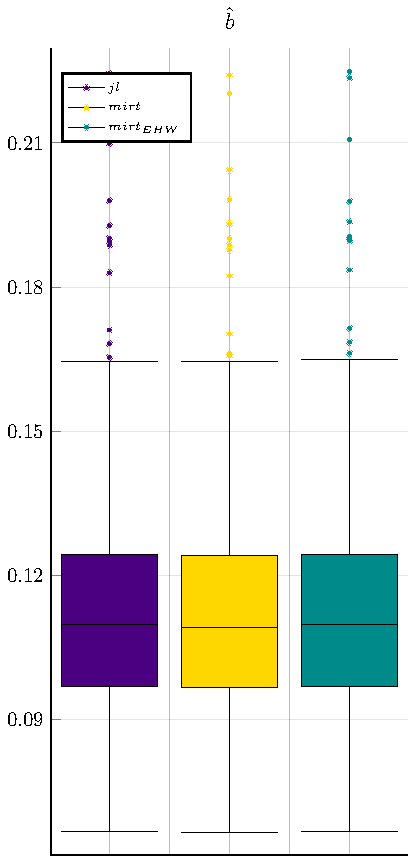
\includegraphics[height=270px,width=.30\textwidth]{Figures/1a/RMSE_b.pdf} & 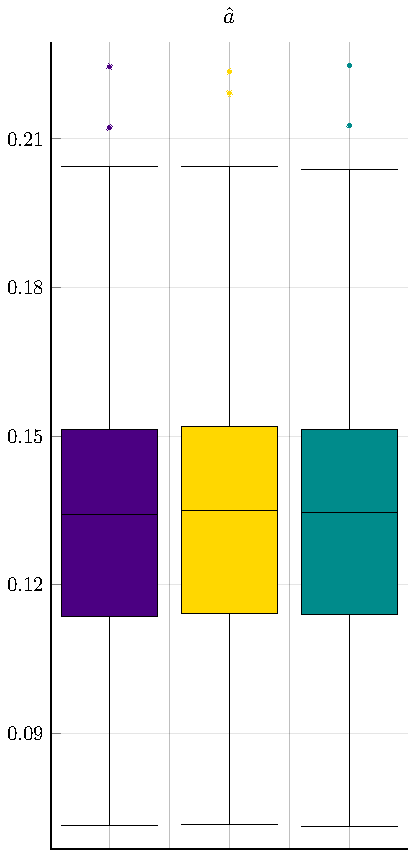
\includegraphics[height=270px,width=.30\textwidth]{Figures/1a/RMSE_a.pdf} & 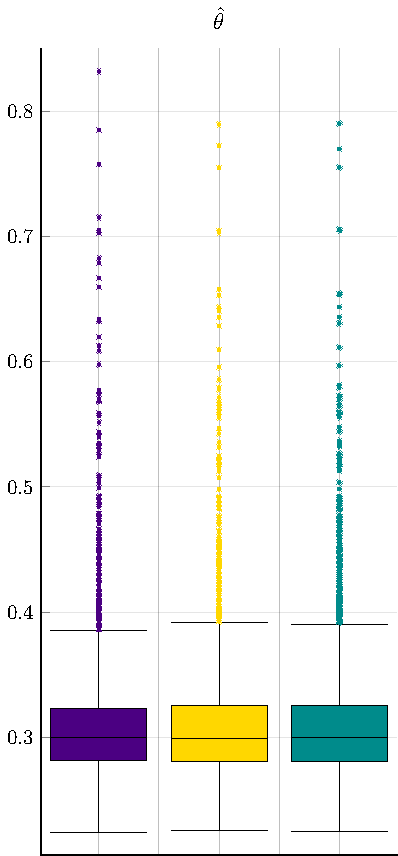
\includegraphics[height=270px,width=.30\textwidth]{Figures/1a/RMSE_t.pdf}
	\end{tabular}
\end{figure}
\begin{figure}[h]
	\centering
	\begin{tabular}[b]{c c c}
		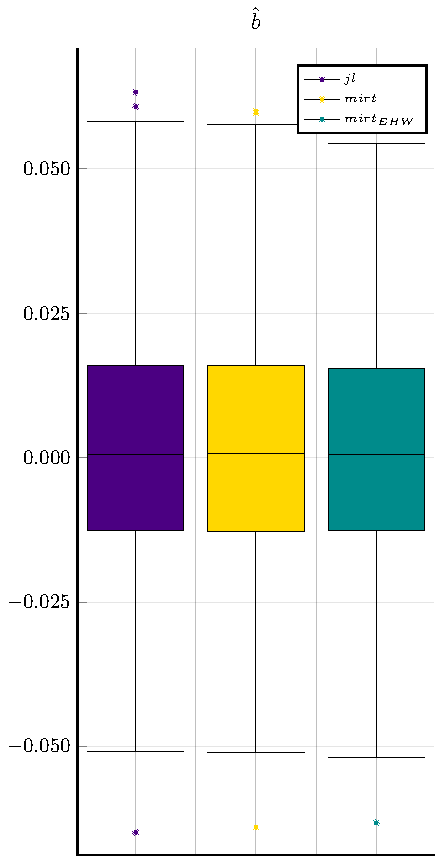
\includegraphics[height=270px,width=.30\textwidth]{Figures/1a/BIAS_b2.pdf} & 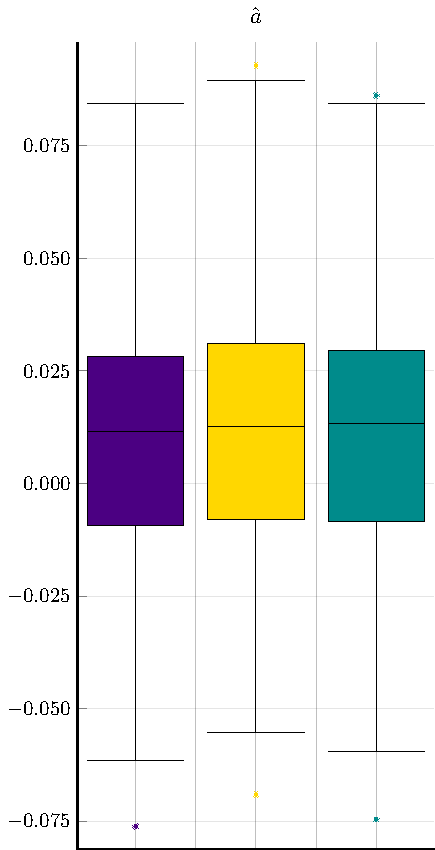
\includegraphics[height=270px,width=.30\textwidth]{Figures/1a/BIAS_a.pdf} & 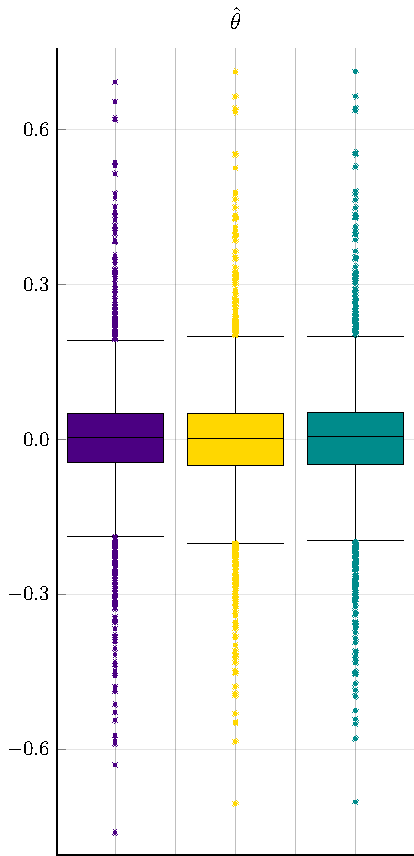
\includegraphics[height=270px,width=.30\textwidth]{Figures/1a/BIAS_t.pdf}
	\end{tabular}
\end{figure}

\subsubsection{Cubic-spline interpolation/extrapolation}

\begin{figure}[h]
	\centering
	\begin{tabular}[b]{c c }
				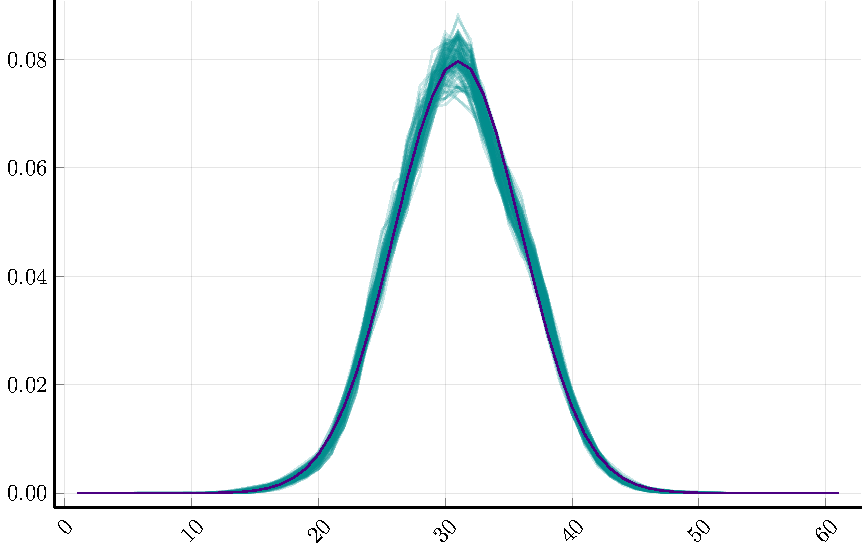
\includegraphics[width=.50\textwidth]{Figures/1a/W.pdf} & 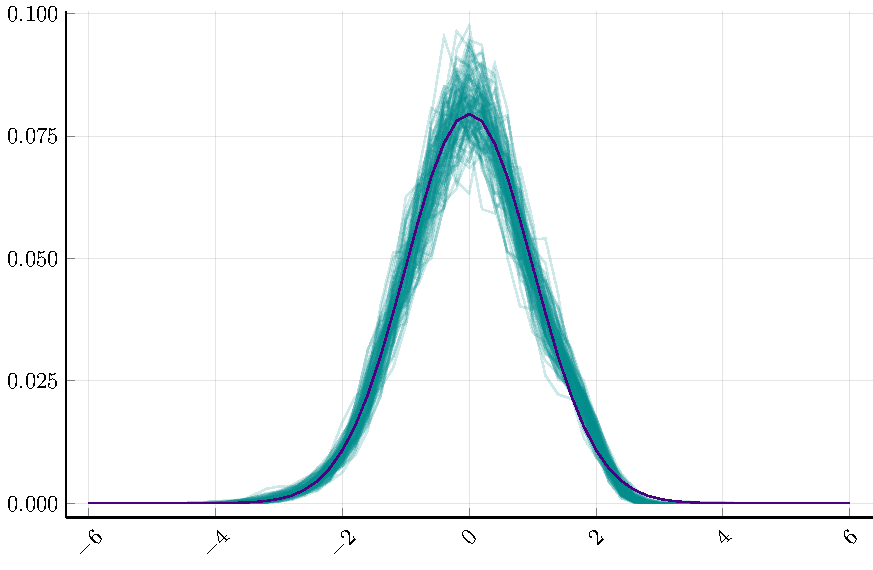
\includegraphics[width=.50\textwidth]{Figures/1b/W.pdf} \\ 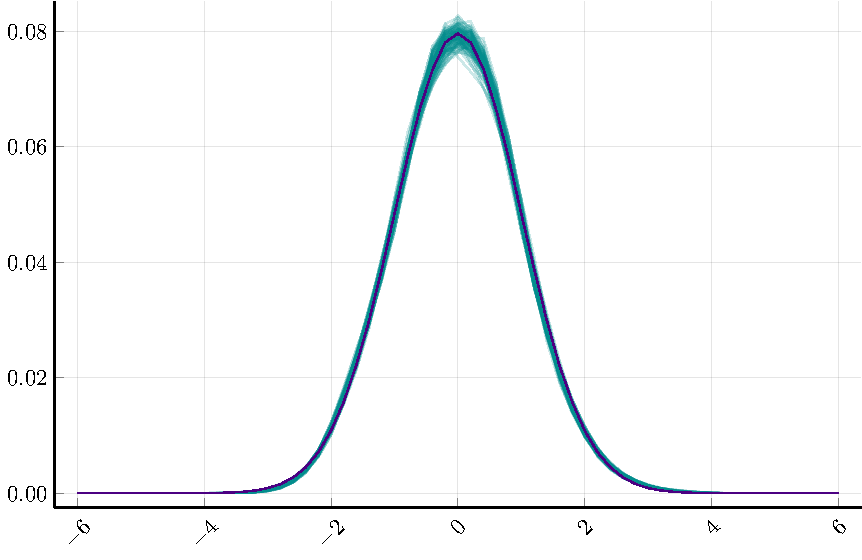
\includegraphics[width=.50\textwidth]{Figures/1c/W.pdf} &		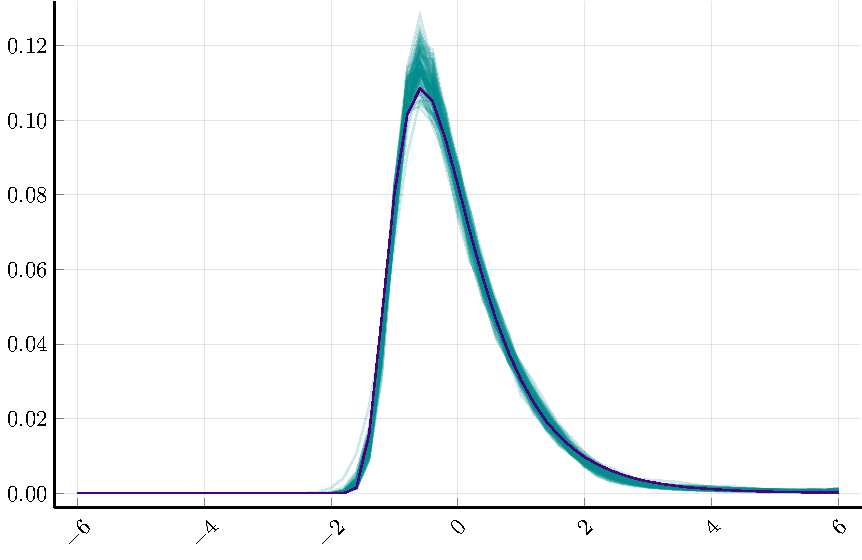
\includegraphics[width=.50\textwidth]{Figures/2a/W.pdf} \\
		 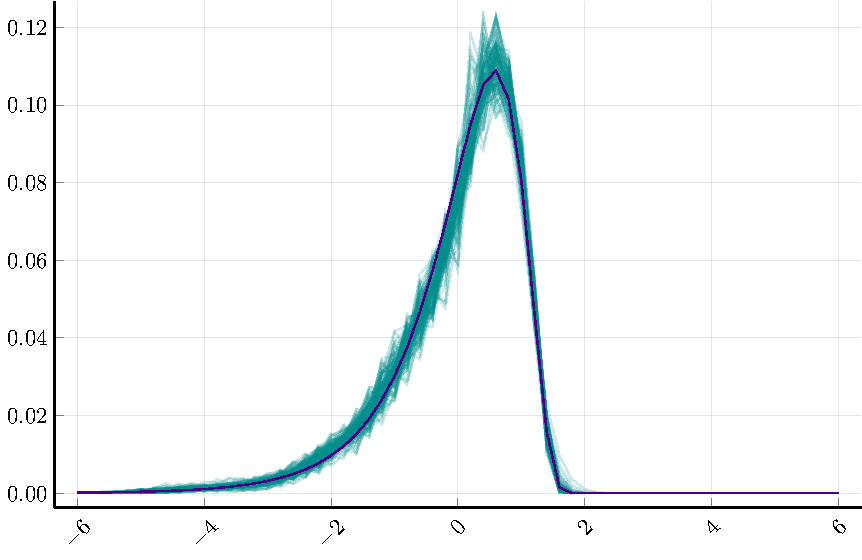
\includegraphics[width=.50\textwidth]{Figures/2b/W.pdf} & 
		 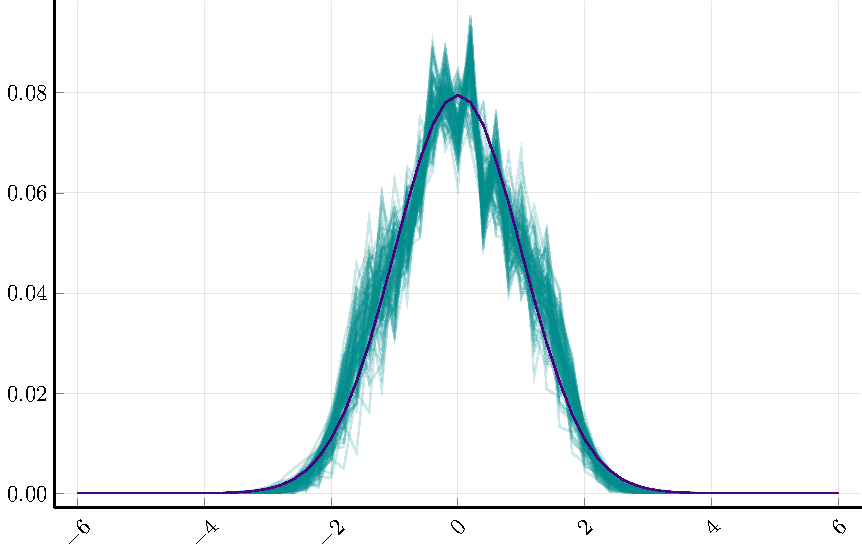
\includegraphics[width=.50\textwidth]{Figures/3/W.pdf}\\
		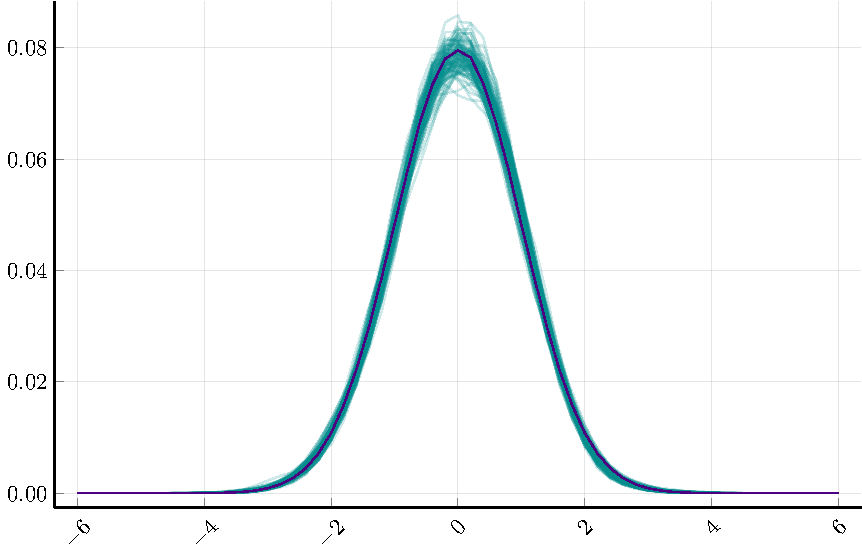
\includegraphics[width=.50\textwidth]{Figures/4/W.pdf} &    \\
	\end{tabular}
	%\textbf{Distribution of RMSEs of estimates across items and test-takers }\par\medskip

	\caption{Retrieval of the latent probability distribution by cubic-spline}
	\label{fig:cubicspline}
\end{figure}


\subsubsection{Computational performance}


To compare the performance of the three considered algorithms, we evaluate their CPU times, and the iteration counts averaged across the $S$ simulations. The results for the cases under analysis are summarized in the following table:

\begin{table}[h]
	\label{tab:cases}
	\renewcommand{\arraystretch}{1.5}%
	\centering
	\caption{Computational power summary}
	\begin{tabular}{ l  c c  c  c c c  }
		& \multicolumn{3}{c}{average CPU time} & \multicolumn{3}{c}{average iterations count} \\
		\toprule
		& {jl} &{mirt} & {mirt\tiny{EHW}} & {jl} &{mirt} & {mirt\tiny{EHW}}  \\
		\midrule
		1a    &\textbf{5.75} & 11.90 &17.27 &88.88 & 55.12  & 59.99  \\%[5pt]
		1b    &\textbf{2.55}  & 9.137 &16.75 & 109.54  &51.31 & 69.12 \\%[2pt]
		1c    &\textbf{10.58}  &14.69  & 20.50 & 92.73 &56.42 & 59.31\\%[2pt]
		2a    & \textbf{7.75}  &12.32 & 21.39 &105.85  & 47.09 & 65.43 \\%[5pt]
		2b    &\textbf{5.77}  & 9.47 & 97.42 & 97.35 & 49.87 & 169.73\\%[5pt]
		3    & \textbf{12.81} & 24.81 &37.54 & 222.28  & 140.44 & 151.14\\%[5pt]
		4    & \textbf{3.59} & 12.98  &16.45  &58.17  &43.86  &53.61 \\%[5pt]
		\bottomrule   
		
	\end{tabular}
	
\end{table}


For the standard setup \texttt{Julia} had a better time performance.
\texttt{Julia} is always faster than the \texttt{mirt EHW} algorithm.
Furthermore, we think that our code is further optimizable by introducing more parallel or distributed computing \texttt{Julia}'s features\footnote{See \url{https://docs.julialang.org/en/v1/manual/parallel-computing/index.html}}.


\subsubsection{Sampling distribution of IRT item parameters}


